\documentclass[tikz,border=10pt]{standalone}
\usepackage{tikz}
\usepackage{unicode-math}
\usetikzlibrary{arrows.meta,decorations.markings}

\begin{document}
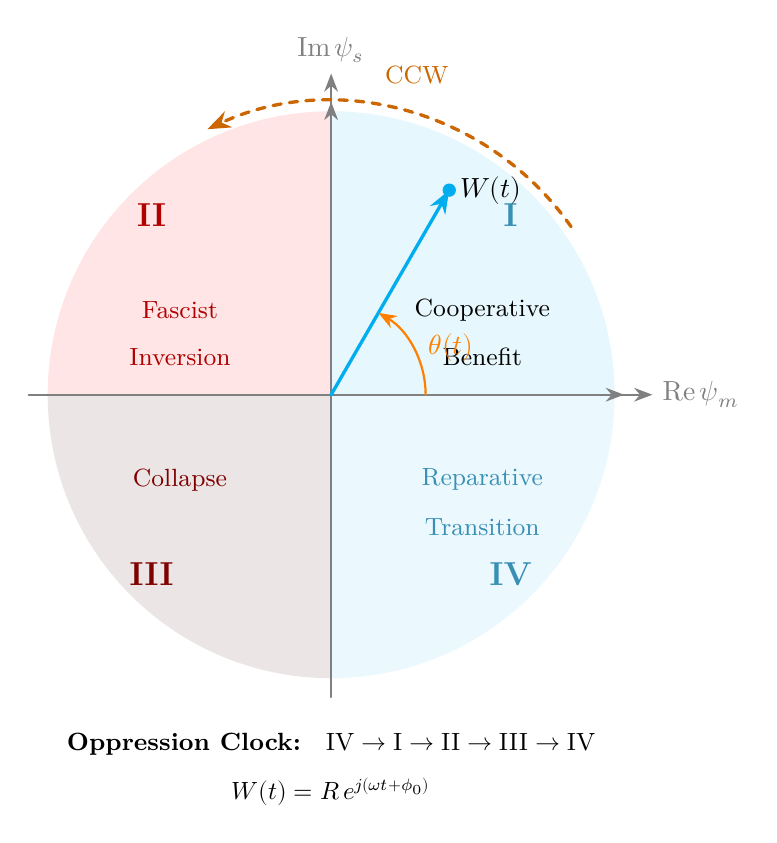
\begin{tikzpicture}[
    >=Stealth,
    line cap=round,
    line join=round,
    scale=1.2
]

% Axes
\draw[->, thick, gray] (-3.2,0) -- (3.4,0) node[right] {$\text{Re}\,\psi_m$};
\draw[->, thick, gray] (0,-3.2) -- (0,3.4) node[above] {$\text{Im}\,\psi_s$};

% Unit circle
\draw[thick, gray!60] (0,0) circle (2.5cm);

% Quadrant backgrounds
\fill[cyan!10] (0,0) -- (3,0) arc (0:90:3) -- cycle;
\fill[red!10] (0,0) -- (0,3) arc (90:180:3) -- cycle;
\fill[red!20!black!10] (0,0) -- (-3,0) arc (180:270:3) -- cycle;
\fill[cyan!8] (0,0) -- (0,-3) arc (270:360:3) -- cycle;

% Axes redrawn on top
\draw[->, thick, gray] (-3.1,0) -- (3.1,0);
\draw[->, thick, gray] (0,-3.1) -- (0,3.1);

% Quadrant labels
\node[font=\bfseries\large, cyan!70!black] at (1.9,1.9) {I};
\node[font=\bfseries\large, red!70!black] at (-1.9,1.9) {II};
\node[font=\bfseries\large, red!50!black] at (-1.9,-1.9) {III};
\node[font=\bfseries\large, cyan!70!black] at (1.9,-1.9) {IV};

% Regime labels
\node[align=center, font=\small] at (1.6,0.9) {Cooperative};
\node[align=center, font=\small] at (1.6,0.4) {Benefit};

\node[align=center, font=\small, red!70!black] at (-1.6,0.9) {Fascist};
\node[align=center, font=\small, red!70!black] at (-1.6,0.4) {Inversion};

\node[align=center, font=\small, red!50!black] at (-1.6,-0.9) {Collapse};

\node[align=center, font=\small, cyan!70!black] at (1.6,-0.9) {Reparative};
\node[align=center, font=\small, cyan!70!black] at (1.6,-1.4) {Transition};

% Phasor arrow at 60 degrees
\draw[->, very thick, cyan] (0,0) -- (60:2.5) node[right, black] {$W(t)$};
\fill[cyan] (60:2.5) circle (2pt);

% Angle arc
\draw[->, thick, orange] (1.0,0) arc (0:60:1.0) node[midway, right, xshift=2pt] {$\theta(t)$};

% CCW rotation arrow (outer)
\draw[->, very thick, orange!80!black, dashed] (35:3.1) arc (35:115:3.1);
\node[font=\small, orange!80!black] at (75:3.5) {CCW};

% Cycle equation at bottom
\node[align=center, font=\small] at (0,-3.7) {\textbf{Oppression Clock:}\quad $\text{IV} \rightarrow \text{I} \rightarrow \text{II} \rightarrow \text{III} \rightarrow \text{IV}$};
\node[align=center, font=\small] at (0,-4.2) {$W(t) = R\,e^{j(\omega t + \phi_0)}$};

\end{tikzpicture}
\end{document}
